\documentclass[tikz,border=5pt]{standalone}
\usepackage{stix2}
\usepackage{xcolor}
\usepackage{tikz}
\usetikzlibrary{arrows.meta, positioning, shapes, calc}

\definecolor{linkblue}{HTML}{004B9B}

\begin{document}

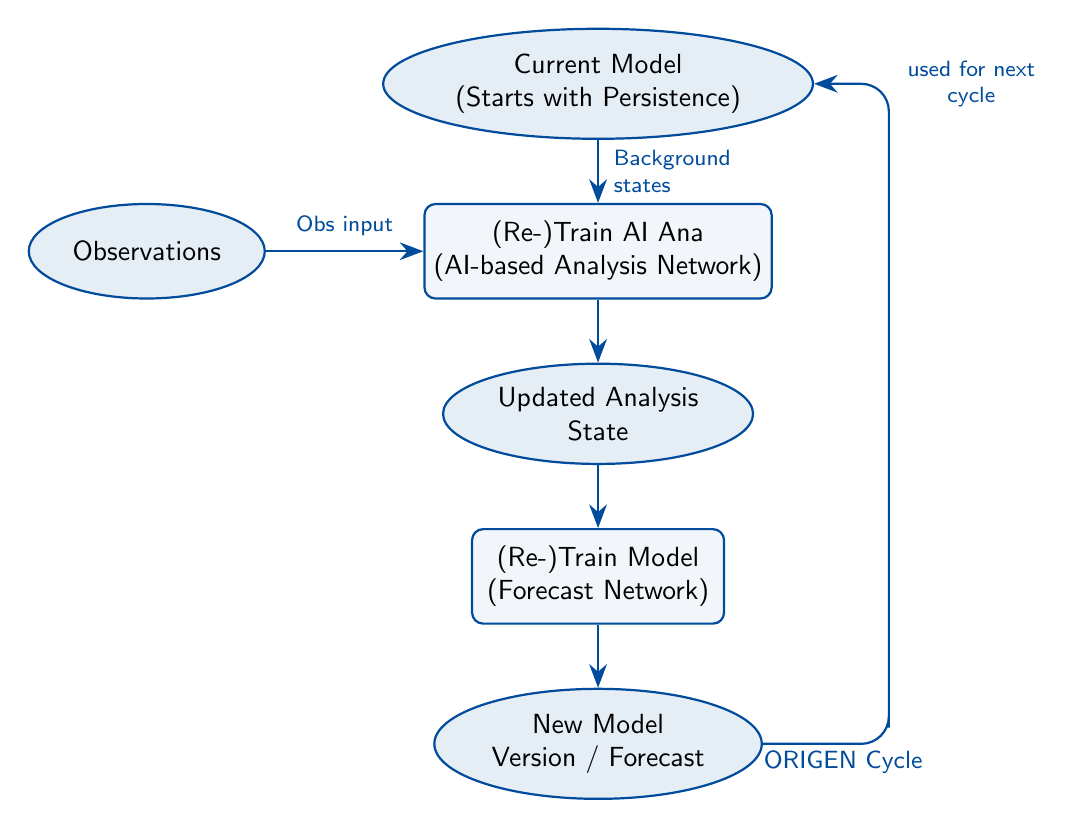
\begin{tikzpicture}[
    node distance=0.8cm and 1.0cm,
    every node/.style={font=\sffamily, align=center},
    process/.style={rectangle, rounded corners, draw=linkblue, thick, fill=linkblue!5,
                    minimum width=3.2cm, minimum height=1.2cm},
    data/.style={ellipse, draw=linkblue, thick, fill=linkblue!10,
                 minimum width=2.8cm, minimum height=1.2cm},
    arrow/.style={-{Stealth[length=3mm]}, thick, linkblue}
]

% --- Nodes ---
\node[data] (model) {Current Model\\(Starts with Persistence)};
\node[process, below=of model] (aida) {(Re-)Train AI Ana\\(AI-based Analysis Network)};
\node[data, below=of aida] (analysis) {Updated Analysis\\State};
\node[process, below=of analysis] (modeltrain) {(Re-)Train Model\\(Forecast Network)};
\node[data, below=of modeltrain] (forecast) {New Model\\Version / Forecast};

% --- Observations input ---
\node[data, left=2cm of aida] (obs) {Observations};

% --- Arrows ---
\draw[arrow] (model) -- node[right=2pt, font=\footnotesize, align=left]{{\sf Background}\\{\sf states}} (aida);
\draw[arrow] (obs) -- node[above=2pt, font=\footnotesize]{{\sf Obs input}} (aida);
\draw[arrow] (aida) -- (analysis);
\draw[arrow] (analysis) -- (modeltrain);
\draw[arrow] (modeltrain) -- (forecast);

% --- Feedback arrow ---
\draw[arrow, rounded corners=10pt]
  (forecast.east) -| ++(1.6,0) |- (model.east)
  node[midway, right=3pt, align=center, font=\footnotesize]{{\sf used for next}\\{\sf cycle}};

% --- Cycle label ---
\node[font=\small, text=linkblue, above right=-1.0cm and 0.5cm of forecast] {{\sf ORIGEN Cycle}};

\end{tikzpicture}

\end{document}
